\section{System Model}
%  \bul{How does a stream processing system operates?} %\incite{8-reqs} %\incite{design-principles}   %
% %dbms vs DSPS Data stream processing systems (DSPS) compute real-time queries over constantly changing
% streams of data. A stream is a possibly infinite sequence of tuples, or timestamped entities.
% Differently than traditional databases, where queries are issued over stored data, in DSPSs queries are
% first submitted to the system, and results are generated continuosly as the new data enters the system
% in the form of streams. This allows the generation of real-time updated results based on the constantly
% changing available data streams.

% sp characteristics
Data Stream Processing Systems (DSPS) have been developed to process large volumes of stream data,
generated in real-time with new values constantly being introduced by the system. Using a traditional
approach of first storing the data and then executing the queries is not appropriate.
The first reason is the amount of available data~\cite{design-principles, 8-reqs}, which is typically
high and potentially too large to be stored entirely by the system.
Another reason not to store all the incoming data is related to its nature: often only a subset of
the data streams are relevant to the application.
Moreover, stream data is transient, with new values constantly updating old ones and rendering
them irrelevant.
Finally, data stream processing also has strict latency constraints and processing data streams with low
latency may be important. Storing the data before processing introduces an unacceptable
delay due to the latency cost of storing and retrieving data on disk.

Figure~\ref{fig:dbms+dsms} shows the two different architectures of a traditional
DBMS (left image) and a DSPS (right image). In the DBMS, queries are issued over previously stored data.
Since the data is already in the system, it is possible to create indexes over it in order to reduce the
query execution time. Results are generated from data received by the system \emph{up to the time} when
the query was issued. The picture on the right, instead, depicts a DSPS. Queries are issued over a
continuously changing stream of data. Once the data enters the system, it is matched against the
registered queries to produce the results. Results are generated from the data received by the system
starting \emph{from the time} when the query was first registered.

\begin{figure}[t!] \centering 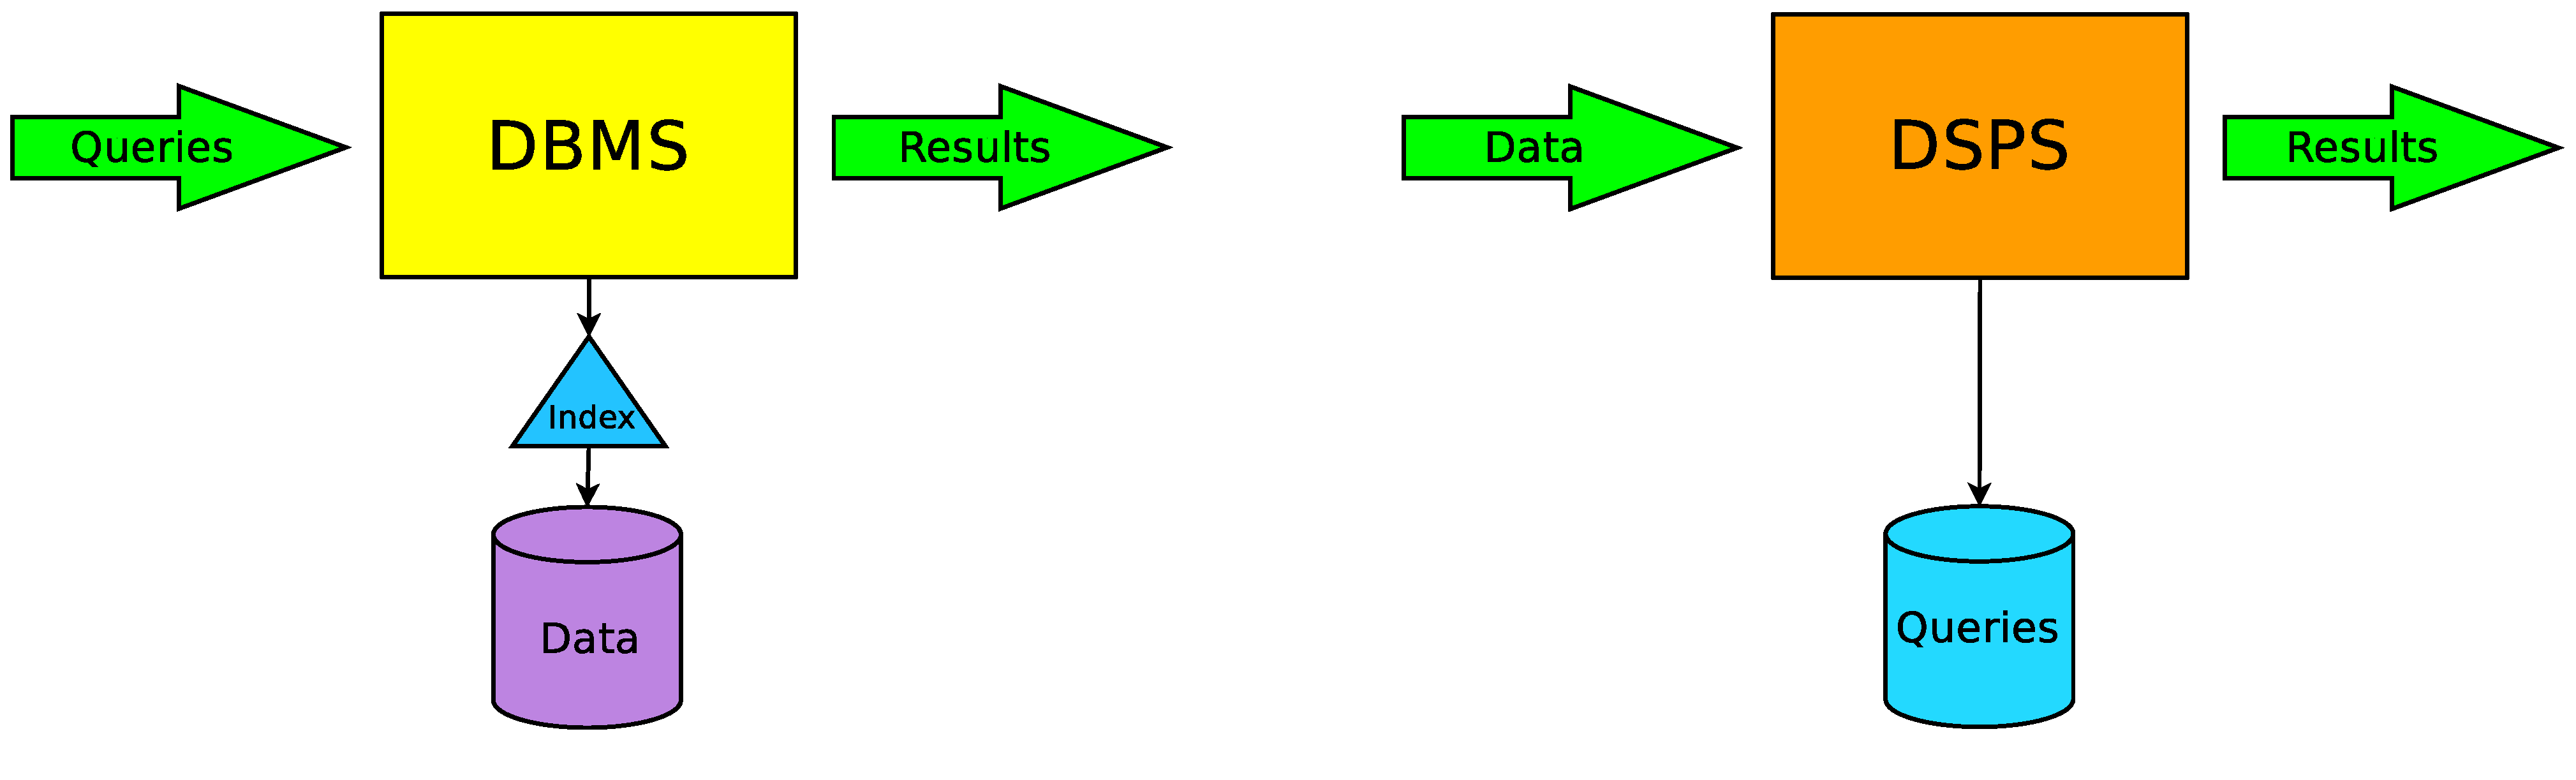
\includegraphics[width=\textwidth]{img/tesi/dbms+dsms} \caption{Comparison
between a traditional Data Base Management System (DBMS) and a Data Stream Processing System (DSPS). On
the left, queries are issued over stored data, while, on the right, data flows through continuous
queries.}
\label{fig:dbms+dsms}
\end{figure}

% \subsubsection*{Issues and Challenges}  \incite{stream-processing-challanges}
% \incite{ds-models-and-issues} \incite{dsm-issues}  \gap
\subsection*{Centralised Architectures}

The first generation of stream processing systems was centralised, with one processing node handling all
the computation. Examples of such systems are STREAM and Aurora.

STREAM~\cite{stream, stream-babcock, stream-chains} is a centralised DSPS, which tries to address the
issue of long-running continuous queries. It uses the relational Continuous Query
Language~(CQL)~\cite{cql} and supports SQL-like queries over continuous data
streams (see~Section~\ref{sec:cql}).
Once a query is registered in the system, a corresponding \textit{query plan} is derived from it.
Query plans are composed of \textit{operators}, which perform the actual processing, \textit{queues},
which buffer tuples as they move between operators, and \textit{synopses}, which store operator state.
All queries are expressed in CQL and then converted into an actual query plan which consists of these
basic elements.
In contrast Aurora~\cite{aurora} introduced the boxes-and-arrows model for queries. Operators are
regarded as boxes, with an input, an output and a specific processing semantic. They are linked
together by arrows representing the stream of tuples flowing between them.
			
\subsection*{Distributed Architectures}
% good replication
The natural step in the evolution of DSPSs is distribution. Centralised systems are inherently subject to
scalability issues. Distributing the processing over a number of nodes is the logical
approach to overcome this issue.
Distribution also allows for better dependability because operators can be replicated at different
locations, thus increasing availability. Fault-tolerance can also be achieved better by employing
distribution because different replicas of operators can be deployed, which achieves resilience to
failure.
The overall performance of the system is also increased by this approach because the computation can be
partitioned and run in parallel at different computing nodes. \\
Distribution can be realised at different scales. Processing nodes can be located within the same data
centre, taking advantage of the high bandwidth and low latency typical of these environments, or spread
out over wide-area networks to push scalability even further.

% issues
Distribution presents several advantages but it comes at a cost. Many issues arise when the system
is distributed: the operational complexity of the system increases and resources need to be allocated
efficiently. In a DSPS, distribution is achieved by partitioning the query plan and running clusters of
operators at different sites. Placing these operators correctly at deployment time and moving them at run time to rebalance the
system are not easy tasks. Running replicas can help increase the dependability of
the system but their correct management represents a key issue.

% systems
Building on the experience of Aurora, a centralised DSPS, other systems have been developed to explore
the possibilities offered by distribution. Aurora*~\cite{aurora*} is an evolution of the Aurora system
that provides interconnection among multiple Aurora instances running in a cluster environment.
A similar example is Medusa~\cite{aurora-and-medusa}, which expands the boundaries of
distribution outside a single cluster onto different processing sites administered by different
authorities.
Borealis~\cite{borealis-design} realises these experiences into a complete distributed
stream processing system. Borealis has been used to explore many research questions related to resource
allocation, \mbox{load-shedding} and replica management. In the following sections, we cover these
topics in more detail.
%  \incite{borBoreealis-design} \incite{mortar-short} \incite{mortar-long} \incite{ss-spc}
\vspace{-10pt}
\subsection*{Operator Placement and Load Balancing}
% op placement is difficult
The optimal distribution of streaming operators over a number of machines is key to maximise the
performance of a distributed stream processing system. Once a query plan has been divided into
clusters, these need to be mapped to available physical computing sites. A placement algorithm
assigns operators to processing nodes while satisfying a set of constraints and attempts to optimise some
objective function. Finding the optimal assignment among the total possible assignments is an NP-hard
problem and thus computationally intractable~\cite{npc-placement}. Despite this, many strategies have
been devised for efficient operator placement and, depending on the assumptions and requirements of the
system, different approaches are more suitable than others. A taxonomy of various placement strategies
for operators can be found in~\cite{placement_strategies}.

% load-balancing
Closely tied to operator placement is the problem of load balancing. While the former is more concerned
with the placement at deployment time, load balancing has to deal with the movement of operators at run
time. During the execution of a query, the amount of data carried by a stream can greatly vary. This may
result in computational overload at some nodes. To recover from this overload condition, the system can
decide to migrate certain operators to a better location, attempting to balance the load among the
available resources. Many operator placement algorithms recognise the need for placement reconfiguration
at run time and make load balancing a key component of their strategy.

% centralized
When the processing nodes of a DSPS are located within the same data centre, the topology management can
be performed by a centralised placement controller. In such environments, the controller can be
aware of the current state of the entire network, including workload information and resource
availability. Having access to this information allows it to reason about placement choices, with results
that are potentially optimal for small deployments. When the number of available resources becomes large
though, such an approach suffers from low scalability. Abadi et al.~\cite{borealis-design} describe
an approach which assumes a fairly constant workload and a heavy cost for operator migration. Xing et
al.~\cite{borealis-xing_placement} consider the workload to be highly unpredictable, thus requiring load
balancing at runtime. They also acknowledge the importance of initial placement and assume a high
migration cost for operators, thus developing an algorithm resilient to load variations~\cite{borealis-load}.
All these algorithms have been implemented within the Borealis DSPS.

% decentralized
When processing nodes are distributed over wide-area networks, a central coordinator becomes
ineffective and a decentralised approach to the problem is more appropriate. Such algorithms make
decisions based on local workload and resource information. Pietzuch et al.~\cite{sbon} propose a
distributed algorithm based on spring relaxation, to minimise a global metric called network usage based
on both bandwidth and latency. Another approach has been taken by Amini et al.~\cite{extreme-scale-sps}.
In this case, an algorithm maximises the weighted throughput of processing elements, while ensuring
stable operation in the face of highly bursty workloads. Zhou et al.~\cite{placement-zhou} propose an
algorithm, in which the initial deployment is determined through minimisation of the communication cost
among processing nodes. It then adapts to the changes in the data and workload within the system. Ying
et al.~\cite{placement-ying} propose to account for the state of operators when performing migration
decisions. When the resources are administered by multiple authorities, the degree of trust and
collaboration among them must be taken into account.
The algorithm from Balazinska et al.~\cite{medusa-load} achieves this by means of pre-negotiated
load-exchange contracts between nodes.
% \subsection*{Resource Allocation}  \subsubsection*{Cluster} \incite{placement-ying}
% \incite{placement-zhou} \incite{borealis-xing_placement} \incite{borealis-load_management}
% \incite{borealis-load}
% 					\incite{medusa-load}
% 					\incite{partial-fault-tolerance}
% 					
% \subsubsection*{Wide-Area}
% 
% 					\incite{sbon}
% 					\incite{placement_strategies} 
% 					\incite{streamglobe}
% 					\incite{adaptive-overlays}
% 					\incite{adaptive-query-deployment}
% 					\incite{adaptive-tree-reorganization}
